\begin{figure}[H]
    \centering
    
\includegraphics[width=0.8\linewidth]{images/DBscan/dbscan_from_scratch_analysis.png}
    \caption{Analysis of DBSCAN clustering implemented from scratch.}
    \label{fig:dbscan_from_scratch_analysis}
\end{figure}

\begin{figure}[H]
    \centering
    
\includegraphics[width=0.8\linewidth]{images/DBscan/dbscan_pca_ground_truth.png}
    \caption{DBSCAN clustering results after PCA, compared to ground truth.}
    \label{fig:dbscan_pca_ground_truth}
\end{figure}

\begin{figure}[H]
    \centering
    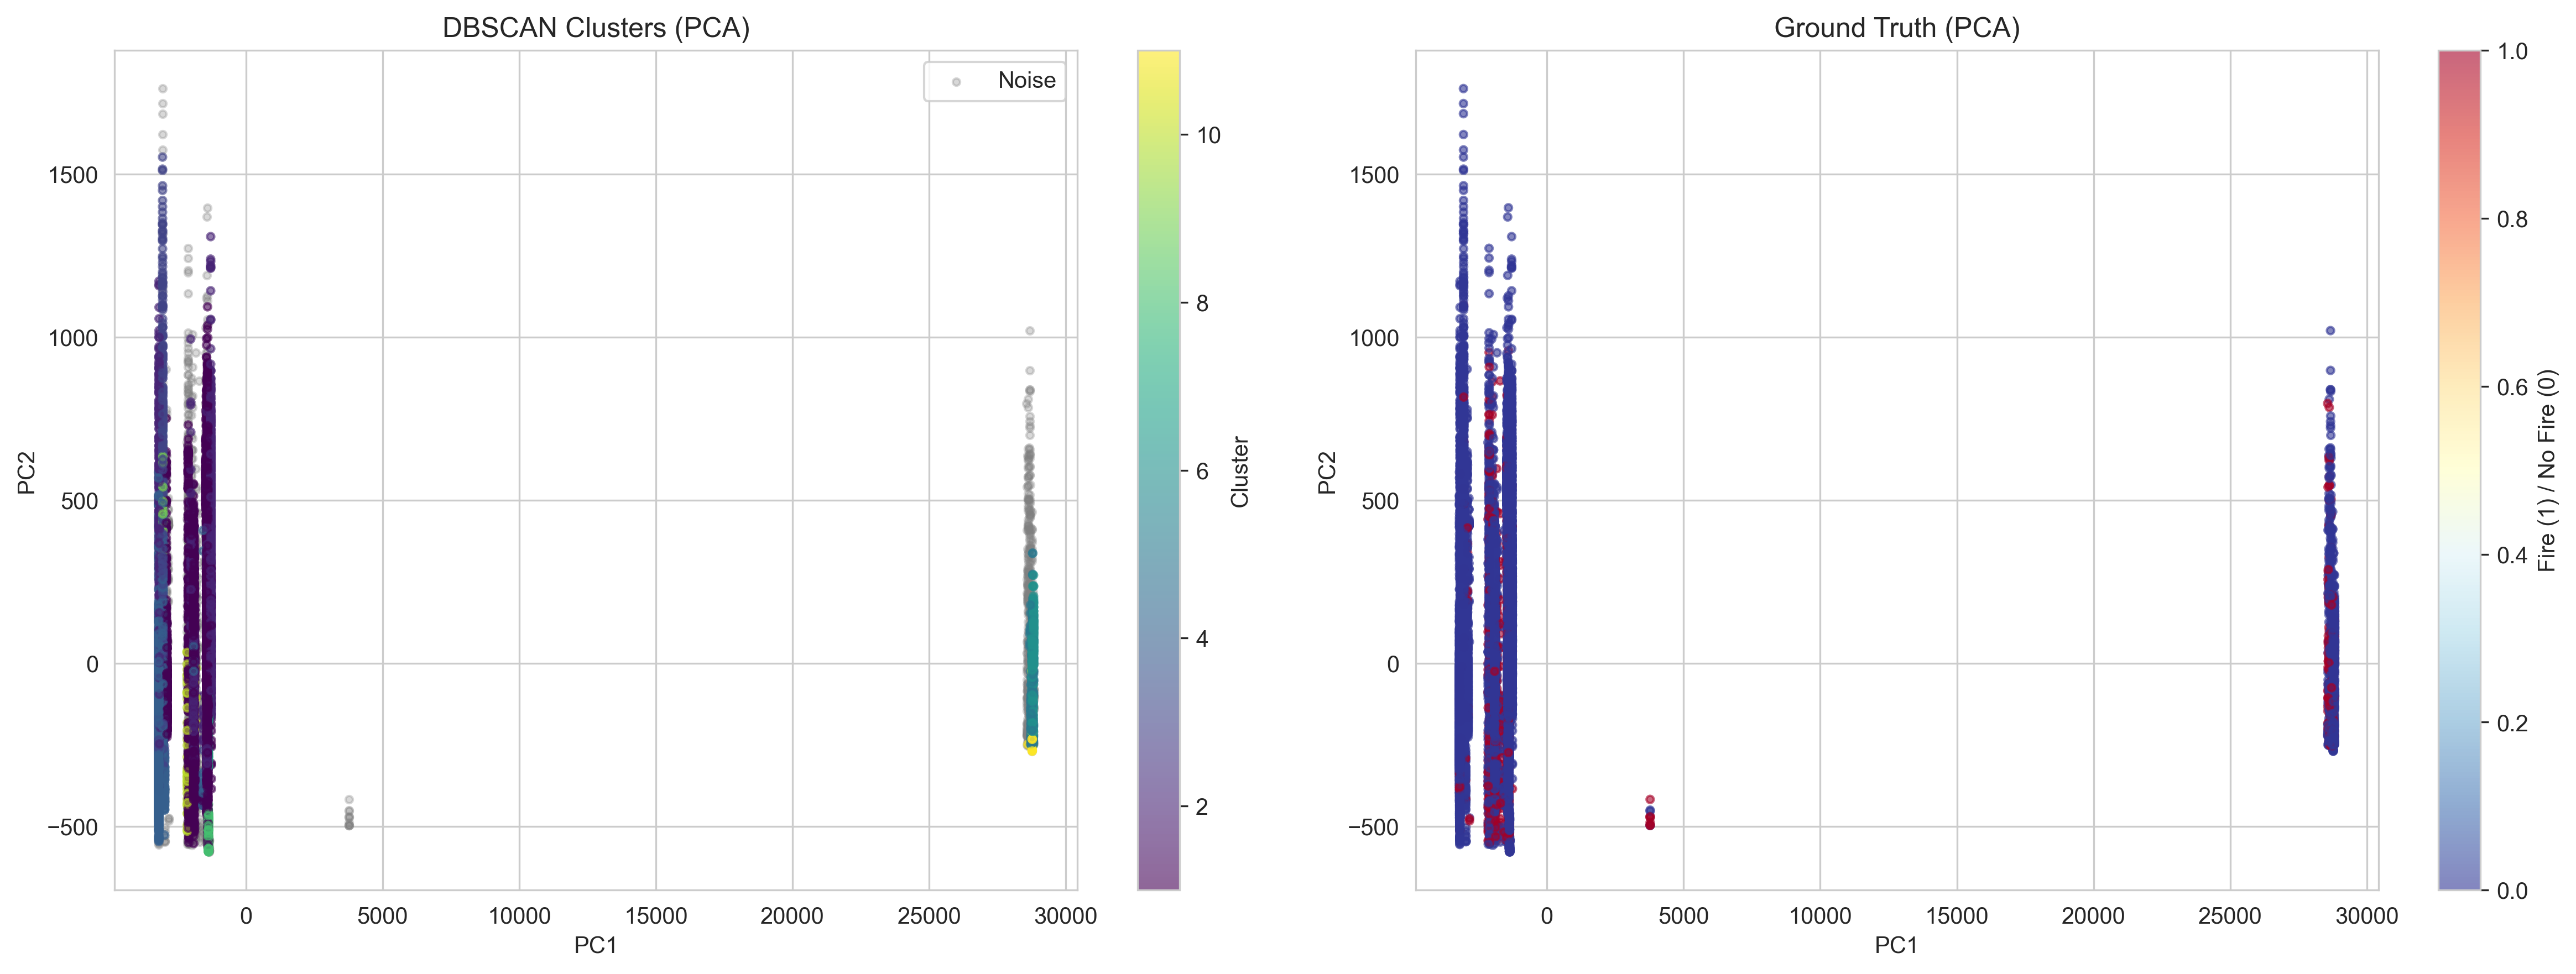
\includegraphics[width=0.8\linewidth]{images/DBscan/dbscan_pca_ground_truth_from_scratch.png}
    \caption{DBSCAN clustering from scratch after PCA, compared to ground truth.}
    \label{fig:dbscan_pca_ground_truth_from_scratch}
\end{figure}

\begin{figure}[H]
    \centering
    
\includegraphics[width=0.8\linewidth]{images/DBscan/dbscan_sklearn_analysis.png}
    \caption{Analysis of DBSCAN clustering using scikit-learn implementation.}
    \label{fig:dbscan_sklearn_analysis}
\end{figure}

\begin{figure}[H]
    \centering
    
\includegraphics[width=0.8\linewidth]{images/DBscan/dbscan_bayesian_optimization.png}
    \caption{Bayesian optimization applied to DBSCAN hyperparameters.}
    \label{fig:dbscan_bayesian_optimization}
\end{figure}
